\documentclass[twoside]{book}

% Packages required by doxygen
\usepackage{fixltx2e}
\usepackage{calc}
\usepackage{doxygen}
\usepackage[export]{adjustbox} % also loads graphicx
\usepackage{graphicx}
\usepackage[utf8]{inputenc}
\usepackage{makeidx}
\usepackage{multicol}
\usepackage{multirow}
\PassOptionsToPackage{warn}{textcomp}
\usepackage{textcomp}
\usepackage[nointegrals]{wasysym}
\usepackage[table]{xcolor}

% Font selection
\usepackage[T1]{fontenc}
\usepackage[scaled=.90]{helvet}
\usepackage{courier}
\usepackage{amssymb}
\usepackage{sectsty}
\renewcommand{\familydefault}{\sfdefault}
\allsectionsfont{%
  \fontseries{bc}\selectfont%
  \color{darkgray}%
}
\renewcommand{\DoxyLabelFont}{%
  \fontseries{bc}\selectfont%
  \color{darkgray}%
}
\newcommand{\+}{\discretionary{\mbox{\scriptsize$\hookleftarrow$}}{}{}}

% Page & text layout
\usepackage{geometry}
\geometry{%
  a4paper,%
  top=2.5cm,%
  bottom=2.5cm,%
  left=2.5cm,%
  right=2.5cm%
}
\tolerance=750
\hfuzz=15pt
\hbadness=750
\setlength{\emergencystretch}{15pt}
\setlength{\parindent}{0cm}
\setlength{\parskip}{3ex plus 2ex minus 2ex}
\makeatletter
\renewcommand{\paragraph}{%
  \@startsection{paragraph}{4}{0ex}{-1.0ex}{1.0ex}{%
    \normalfont\normalsize\bfseries\SS@parafont%
  }%
}
\renewcommand{\subparagraph}{%
  \@startsection{subparagraph}{5}{0ex}{-1.0ex}{1.0ex}{%
    \normalfont\normalsize\bfseries\SS@subparafont%
  }%
}
\makeatother

% Headers & footers
\usepackage{fancyhdr}
\pagestyle{fancyplain}
\fancyhead[LE]{\fancyplain{}{\bfseries\thepage}}
\fancyhead[CE]{\fancyplain{}{}}
\fancyhead[RE]{\fancyplain{}{\bfseries\leftmark}}
\fancyhead[LO]{\fancyplain{}{\bfseries\rightmark}}
\fancyhead[CO]{\fancyplain{}{}}
\fancyhead[RO]{\fancyplain{}{\bfseries\thepage}}
\fancyfoot[LE]{\fancyplain{}{}}
\fancyfoot[CE]{\fancyplain{}{}}
\fancyfoot[RE]{\fancyplain{}{\bfseries\scriptsize Generated by Doxygen }}
\fancyfoot[LO]{\fancyplain{}{\bfseries\scriptsize Generated by Doxygen }}
\fancyfoot[CO]{\fancyplain{}{}}
\fancyfoot[RO]{\fancyplain{}{}}
\renewcommand{\footrulewidth}{0.4pt}
\renewcommand{\chaptermark}[1]{%
  \markboth{#1}{}%
}
\renewcommand{\sectionmark}[1]{%
  \markright{\thesection\ #1}%
}

% Indices & bibliography
\usepackage{natbib}
\usepackage[titles]{tocloft}
\setcounter{tocdepth}{3}
\setcounter{secnumdepth}{5}
\makeindex

% Hyperlinks (required, but should be loaded last)
\usepackage{ifpdf}
\ifpdf
  \usepackage[pdftex,pagebackref=true]{hyperref}
\else
  \usepackage[ps2pdf,pagebackref=true]{hyperref}
\fi
\hypersetup{%
  colorlinks=true,%
  linkcolor=blue,%
  citecolor=blue,%
  unicode%
}

% Custom commands
\newcommand{\clearemptydoublepage}{%
  \newpage{\pagestyle{empty}\cleardoublepage}%
}

\usepackage{caption}
\captionsetup{labelsep=space,justification=centering,font={bf},singlelinecheck=off,skip=4pt,position=top}

%===== C O N T E N T S =====

\begin{document}

% Titlepage & ToC
\hypersetup{pageanchor=false,
             bookmarksnumbered=true,
             pdfencoding=unicode
            }
\pagenumbering{roman}
\begin{titlepage}
\vspace*{7cm}
\begin{center}%
{\Large L\+AB \\[1ex]\large 5 }\\
\vspace*{1cm}
{\large Generated by Doxygen 1.8.11}\\
\end{center}
\end{titlepage}
\clearemptydoublepage
\tableofcontents
\clearemptydoublepage
\pagenumbering{arabic}
\hypersetup{pageanchor=true}

%--- Begin generated contents ---
\chapter{Class Index}
\section{Class List}
Here are the classes, structs, unions and interfaces with brief descriptions\+:\begin{DoxyCompactList}
\item\contentsline{section}{\hyperlink{classPrimo}{Primo} }{\pageref{classPrimo}}{}
\end{DoxyCompactList}

\chapter{File Index}
\section{File List}
Here is a list of all documented files with brief descriptions\+:\begin{DoxyCompactList}
\item\contentsline{section}{src/questao\+\_\+1/\hyperlink{main__q1_8cpp}{main\+\_\+q1.\+cpp} \\*Questao\+\_\+1 -\/ L\+A\+B5 }{\pageref{main__q1_8cpp}}{}
\item\contentsline{section}{src/questao\+\_\+2/\hyperlink{main__q2_8cpp}{main\+\_\+q2.\+cpp} \\*Questao\+\_\+2 -\/ L\+A\+B5 }{\pageref{main__q2_8cpp}}{}
\item\contentsline{section}{src/questao\+\_\+3/\hyperlink{main__q3_8cpp}{main\+\_\+q3.\+cpp} \\*Showprimos -\/ L\+A\+B5 }{\pageref{main__q3_8cpp}}{}
\end{DoxyCompactList}

\chapter{Class Documentation}
\hypertarget{classPrimo}{}\section{Primo Class Reference}
\label{classPrimo}\index{Primo@{Primo}}
\subsection*{Public Member Functions}
\begin{DoxyCompactItemize}
\item 
{\bfseries Primo} (int number)\hypertarget{classPrimo_ae5a273f531a2b0b1654744d3e13a5d4d}{}\label{classPrimo_ae5a273f531a2b0b1654744d3e13a5d4d}

\item 
bool {\bfseries operator()} (int n) const \hypertarget{classPrimo_acd6a2d019b6bd33cc1282ea895223276}{}\label{classPrimo_acd6a2d019b6bd33cc1282ea895223276}

\end{DoxyCompactItemize}


The documentation for this class was generated from the following file\+:\begin{DoxyCompactItemize}
\item 
src/questao\+\_\+3/\hyperlink{main__q3_8cpp}{main\+\_\+q3.\+cpp}\end{DoxyCompactItemize}

\chapter{File Documentation}
\hypertarget{main__q1_8cpp}{}\section{src/questao\+\_\+1/main\+\_\+q1.cpp File Reference}
\label{main__q1_8cpp}\index{src/questao\+\_\+1/main\+\_\+q1.\+cpp@{src/questao\+\_\+1/main\+\_\+q1.\+cpp}}


Questao\+\_\+1 -\/ L\+A\+B5.  


{\ttfamily \#include $<$iostream$>$}\\*
{\ttfamily \#include $<$vector$>$}\\*
Include dependency graph for main\+\_\+q1.\+cpp\+:
\nopagebreak
\begin{figure}[H]
\begin{center}
\leavevmode
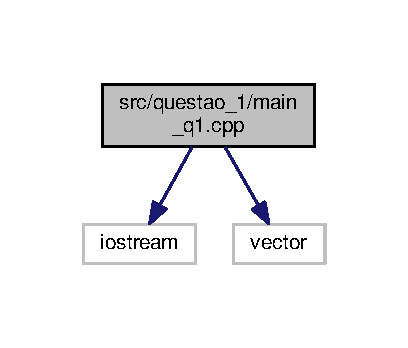
\includegraphics[width=196pt]{main__q1_8cpp__incl}
\end{center}
\end{figure}
\subsection*{Functions}
\begin{DoxyCompactItemize}
\item 
{\footnotesize template$<$typename Input\+Iterator $>$ }\\Input\+Iterator \hyperlink{main__q1_8cpp_af819425965e300c89f2a7eddbcf3835d}{closest2mean} (Input\+Iterator first, Input\+Iterator last)
\begin{DoxyCompactList}\small\item\em Função que recebe um Iterador genérico utilizando templates. \end{DoxyCompactList}\item 
int {\bfseries main} ()\hypertarget{main__q1_8cpp_ae66f6b31b5ad750f1fe042a706a4e3d4}{}\label{main__q1_8cpp_ae66f6b31b5ad750f1fe042a706a4e3d4}

\end{DoxyCompactItemize}


\subsection{Detailed Description}
Questao\+\_\+1 -\/ L\+A\+B5. 

Utilização de Iteradores Genéricos \begin{DoxyAuthor}{Author}
Ariel Oliveira (\href{mailto:ariel.oliveira01@gmail.com}{\tt ariel.\+oliveira01@gmail.\+com}) 
\end{DoxyAuthor}
\begin{DoxySince}{Since}
31/10/2017 
\end{DoxySince}
\begin{DoxyDate}{Date}
06/11/2017 
\end{DoxyDate}


\subsection{Function Documentation}
\index{main\+\_\+q1.\+cpp@{main\+\_\+q1.\+cpp}!closest2mean@{closest2mean}}
\index{closest2mean@{closest2mean}!main\+\_\+q1.\+cpp@{main\+\_\+q1.\+cpp}}
\subsubsection[{\texorpdfstring{closest2mean(\+Input\+Iterator first, Input\+Iterator last)}{closest2mean(InputIterator first, InputIterator last)}}]{\setlength{\rightskip}{0pt plus 5cm}template$<$typename Input\+Iterator $>$ Input\+Iterator closest2mean (
\begin{DoxyParamCaption}
\item[{Input\+Iterator}]{first, }
\item[{Input\+Iterator}]{last}
\end{DoxyParamCaption}
)}\hypertarget{main__q1_8cpp_af819425965e300c89f2a7eddbcf3835d}{}\label{main__q1_8cpp_af819425965e300c89f2a7eddbcf3835d}


Função que recebe um Iterador genérico utilizando templates. 


\begin{DoxyParams}{Parameters}
{\em Input\+Iterator} & first \\
\hline
{\em Input\+Iterator} & last \\
\hline
\end{DoxyParams}
\begin{DoxyReturn}{Returns}
template typename Input\+Iterator 
\end{DoxyReturn}

\hypertarget{main__q2_8cpp}{}\section{src/questao\+\_\+2/main\+\_\+q2.cpp File Reference}
\label{main__q2_8cpp}\index{src/questao\+\_\+2/main\+\_\+q2.\+cpp@{src/questao\+\_\+2/main\+\_\+q2.\+cpp}}


Questao\+\_\+2 -\/ L\+A\+B5.  


{\ttfamily \#include $<$iostream$>$}\\*
{\ttfamily \#include $<$set$>$}\\*
{\ttfamily \#include $<$vector$>$}\\*
Include dependency graph for main\+\_\+q2.\+cpp\+:
\nopagebreak
\begin{figure}[H]
\begin{center}
\leavevmode
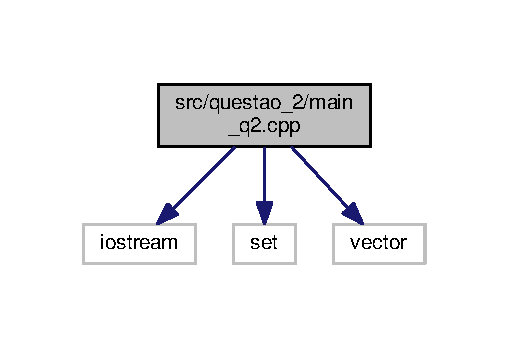
\includegraphics[width=244pt]{main__q2_8cpp__incl}
\end{center}
\end{figure}
\subsection*{Functions}
\begin{DoxyCompactItemize}
\item 
{\footnotesize template$<$typename T\+Container $>$ }\\void \hyperlink{main__q2_8cpp_adf07efaecf4a60b87a8e74210855bd46}{print\+\_\+elements} (const T\+Container \&collection, const char $\ast$label=\char`\"{}\char`\"{}, const char separator=\textquotesingle{} \textquotesingle{})
\begin{DoxyCompactList}\small\item\em Função que recebe uma referência de um Container genérico através de templates. \end{DoxyCompactList}\item 
int {\bfseries main} ()\hypertarget{main__q2_8cpp_ae66f6b31b5ad750f1fe042a706a4e3d4}{}\label{main__q2_8cpp_ae66f6b31b5ad750f1fe042a706a4e3d4}

\end{DoxyCompactItemize}


\subsection{Detailed Description}
Questao\+\_\+2 -\/ L\+A\+B5. 

Exemplo de função que recebe um container genérico, utilizando seus respectivos iteradores através de templates \begin{DoxyAuthor}{Author}
Ariel Oliveira (\href{mailto:ariel.oliveira01@gmail.com}{\tt ariel.\+oliveira01@gmail.\+com}) 
\end{DoxyAuthor}
\begin{DoxySince}{Since}
31/10/2017 
\end{DoxySince}
\begin{DoxyDate}{Date}
06/11/2017 
\end{DoxyDate}


\subsection{Function Documentation}
\index{main\+\_\+q2.\+cpp@{main\+\_\+q2.\+cpp}!print\+\_\+elements@{print\+\_\+elements}}
\index{print\+\_\+elements@{print\+\_\+elements}!main\+\_\+q2.\+cpp@{main\+\_\+q2.\+cpp}}
\subsubsection[{\texorpdfstring{print\+\_\+elements(const T\+Container \&collection, const char $\ast$label="""", const char separator=\textquotesingle{} \textquotesingle{})}{print_elements(const TContainer &collection, const char *label="", const char separator=' ')}}]{\setlength{\rightskip}{0pt plus 5cm}template$<$typename T\+Container $>$ void print\+\_\+elements (
\begin{DoxyParamCaption}
\item[{const T\+Container \&}]{collection, }
\item[{const char $\ast$}]{label = {\ttfamily \char`\"{}\char`\"{}}, }
\item[{const char}]{separator = {\ttfamily \textquotesingle{}~\textquotesingle{}}}
\end{DoxyParamCaption}
)}\hypertarget{main__q2_8cpp_adf07efaecf4a60b87a8e74210855bd46}{}\label{main__q2_8cpp_adf07efaecf4a60b87a8e74210855bd46}


Função que recebe uma referência de um Container genérico através de templates. 


\begin{DoxyParams}{Parameters}
{\em T\+Container\&} & collection \\
\hline
{\em const} & char$\ast$ label=\char`\"{}\char`\"{} \\
\hline
{\em const} & char separator= \textquotesingle{} \textquotesingle{} \\
\hline
\end{DoxyParams}
\begin{DoxyReturn}{Returns}
void 
\end{DoxyReturn}

\hypertarget{main__q3_8cpp}{}\section{src/questao\+\_\+3/main\+\_\+q3.cpp File Reference}
\label{main__q3_8cpp}\index{src/questao\+\_\+3/main\+\_\+q3.\+cpp@{src/questao\+\_\+3/main\+\_\+q3.\+cpp}}


showprimos -\/ L\+A\+B5  


{\ttfamily \#include $<$iostream$>$}\\*
{\ttfamily \#include $<$vector$>$}\\*
{\ttfamily \#include $<$algorithm$>$}\\*
{\ttfamily \#include $<$math.\+h$>$}\\*
Include dependency graph for main\+\_\+q3.\+cpp\+:
\nopagebreak
\begin{figure}[H]
\begin{center}
\leavevmode
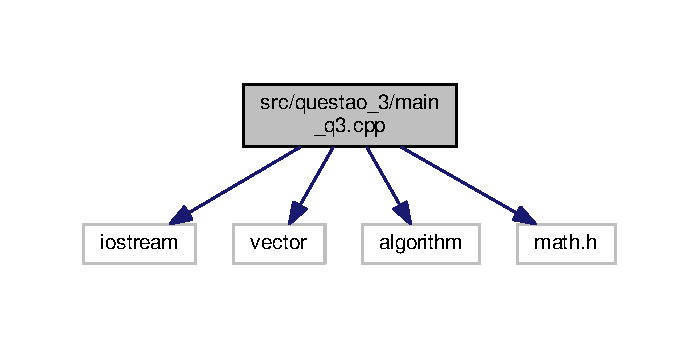
\includegraphics[width=336pt]{main__q3_8cpp__incl}
\end{center}
\end{figure}
\subsection*{Classes}
\begin{DoxyCompactItemize}
\item 
class \hyperlink{classPrimo}{Primo}
\end{DoxyCompactItemize}
\subsection*{Functions}
\begin{DoxyCompactItemize}
\item 
int {\bfseries main} (int argc, char $\ast$$\ast$argv)\hypertarget{main__q3_8cpp_a3c04138a5bfe5d72780bb7e82a18e627}{}\label{main__q3_8cpp_a3c04138a5bfe5d72780bb7e82a18e627}

\end{DoxyCompactItemize}


\subsection{Detailed Description}
showprimos -\/ L\+A\+B5 

Exemplo de utilização de Predicados

Neste exemplo, pede-\/se a implementação de um functor que retorne verdadeiro caso o número seja primo. Utilizando a função find\+\_\+if, da biblioteca algorithm, o programa deverá imprimir todos os números primos de 1 até N \begin{DoxyAuthor}{Author}
Ariel Oliveira (\href{mailto:ariel.oliveira01@gmail.com}{\tt ariel.\+oliveira01@gmail.\+com}) 
\end{DoxyAuthor}
\begin{DoxySince}{Since}
31/10/2017 
\end{DoxySince}
\begin{DoxyDate}{Date}
06/11/2017 
\end{DoxyDate}

%--- End generated contents ---

% Index
\backmatter
\newpage
\phantomsection
\clearemptydoublepage
\addcontentsline{toc}{chapter}{Index}
\printindex

\end{document}
